

\subsection{API}
API steht für Application Programming Interface und bezeichnet eine Programmierschnittstelle für die Kommunikation von Diensten.
Zur einfacheren Handhabung und höherer Flexibilität sollen Daten über einen standardisierten Weg ausgetauscht werden. Die API definiert
dabei die Art und Weise der Kommunikation, also wie Daten angenommen, verarbeitet und wieder zurückgesendet werden.

Für die Webanwendung ist eine API unerlässlich, da der Datenverkehr reguliert werden muss.
Amazon bietet zwei Möglichkeiten an eine solche API zu erstellen.
Zur Auswahl stehen die Amazon Dienste API Gateway und AppSync.
Beide Dienste basieren auf unterschiedlichen Prinzipien mit eigenen Vor- und Nachteilen.
Diese Aspekte werden im folgenden Schritt gegenüber gestellt.
Anschließend folgt anhand der gewonnenen Erkenntnisse eine begründete Entscheidung, welcher Dienst geeigneter ist.

\clearpage
\subsubsection{REST API: AWS API Gateway}
Das Grundprinzip der REST-API (REpresentational State Transfer) Architektur ist es eine strukturierte Kombination aus Ressourcen und Methoden zu erhalten.
Jede Information, die sich benennen lässt kann eine Ressource sein.
Identifiziert werden Ressourcen mithilfe von sogenannten URI (Unified Resource Identifier).
Sie geben Inhalte in JSON oder XML zurück.
Mittels den zustandslosen HTTP-Methoden \verb+GET, POST, PUT+ und \verb+DELETE+ kann mit Servern im Internet agiert werden.
Laut Anforderungen soll sich REST an das Client-Server Modell halten und unabhängig voneinander funktionieren können.
Der Client hat jederzeit die Möglichkeit Daten vom Server anzufordern.
Dabei muss jede Anfrage des Clients alle benötigten Informationen beinhalten um die Anfrage bearbeiten zu können.
Die gewünschten Daten sind immer über eine spezifische URI identifizierbar.
Jede Ressource besitzt eine eigene URI.\cite{REST}

Beispiel für Abfragen könnten folgendermaßen aussehen:

\begin{lstlisting}[basicstyle=\ttfamily, breaklines=true , frame = single, backgroundcolor=\color{flashwhite} ]
GET /AccountNames/
GET /AccountNames/123
GET /AccountNames/456
POST /Accounts/1
\end{lstlisting}

Mithilfe der ersten \verb+GET+ Anfrage kann eine Liste von Accounts abgerufen werden, die zweite \verb+GET+ Anfrage liefert nur die Informationen für den Eintrag \glqq 123\grqq{}  der Accountnamen.
Um nur zwei Namen zu erhalten, sind dementsprechend auch zwei Abfragen notwendig, da sie separate Ressourcen sind.
Eine alternative Option wäre alle Accountnamen zu erhalten und nur die benötigten heraus zu filtern.
Die \verb+POST+ Abfrage erlaubt es einen neuen Account anzulegen.
Es ist wichtig vorher zu überlegen in welchem Kontext die Daten später benötigt werden.
Dank der Zustandslosigkeit wird eine leichtere Skalierung ermöglicht.
Anfragen können durch einen Loadbalancer auf mehrere Server verteilt und bearbeitet werden.

Auch eine Cache-Implementierung ist mithilfe von REST leicht umsetzbar.
Durch Caching werden häufig abgerufene Daten zwischengespeichert.
Ziel ist es die Performance zu steigern und damit gleichzeitig die Anzahl der Abfragen an den Ursprungsserver zu reduzieren.
Stellt zum Beispiel ein Browser eine Anfrage, wird zuerst geschaut, ob sich die benötigten Daten im Cache befinden.
Falls ja werden sie aus dem Cache geliefert und der Server wird nicht kontaktiert.
Fehlen die Daten im Cache werden sie von dem Server abgefragt und anschließend dem Client zurückgegeben und zusätzlich im Cache gespeichert, sodass jede weitere Anfrage direkt aus dem Cache ausgeliefert werden kann.
Der Client stellt seine Anfrage dabei normal an den Zielserver, für ihn ist der Cache nicht direkt sichtbar.
Beim HTTP-Caching entscheidet der \verb+Cache-Control+ Header\footnote{Ein HTTP-Header ist eine Zusatzinformation die zwischen Client und Server ausgetauscht werden kann.} ob und wie lange ein Datensatz als gültig gilt.
Ein gesetzter Header mit dem Wert \verb+Cache-Control: max-age=3600+ teilt dem Client etwa mit, dass die Datei eine Stunde gültig ist, und in diesem Zeitraum nicht erneut abgerufen werden muss. \cite[Seite 21]{Cache}
\clearpage
Wächst eine Applikation immer weiter entstehen auch meist neue API Endpunkte.
Besteht die Anforderung alle Daten abzufragen, wären mehrere separate Anfragen notwendig.
Es ist zudem nicht möglich die angeforderten Daten genauer zu spezifizieren.
Mittels \verb+GET+ Abfrage erhält man immer alle Daten, die die API zurückgibt, egal wie viel man tatsächlich davon benötigt.
Dieses Phänomen nennt sich Over-fetching bzw. Under-fetching.
Beim Over-fetching werden mehr Daten bezogen als die Anwendung eigentlich benötigt und beim Under-fetching müssen mehrere Anfragen an den Server gesendet werden um die benötigte Menge an Daten zu erhalten.\cite{API}

AWS API Gateway ist ein vollständig verwalteter Service, der solche API-Endpunkte erzeugt.
Dabei steht er als zentrale Schnittstelle zwischen Endgeräten und Backend-Diensten.
Zu den Endgeräten zählen Webanwendungen, Mobilgeräte oder auch
IoT\footnote{IoT steht für Internet of Things (deutsch: Internet der Dinge) und bezeichnet ein System von vernetzten Geräten, welche
 über das Internet miteinander kommunizieren können. Dazu gehören Geräte die ihre Daten selbständig sammeln und zur Verfügung stellen können,
 etwa auch Alltagsgegenstände wie smarte Thermostate oder digitale Sprachassistenten. } Geräte.
Eingehende Abfragen werden mit API Gateway an einen ausgewählten Dienst weitergeleitet.
Für jede unterschiedliche Abfrage lässt sich ein anderes Verhalten konfigurieren.
Mithilfe des Dienstes lässt sich beispielhaft die zuvor beschriebene \verb+GET+ Abfrage an eine Datenbank weiterleiten, die die gewünschten Daten zurückgibt.
Die \verb+POST+ Abfrage könnte an eine Lambda-Funktion weitergeleitet werden, welche die Daten verarbeitet und an einem anderen Ort speichert.
AWS API Gateway arbeitet dabei vollkommen Serverless und skaliert automatisch mit den Anforderungen. Neben Zugriff auf den Lambda-Dienst, ist es auch möglich
mit anderen Diensten wie EC2, S3 oder auch DynamoDB (siehe \textit{\ref{DynamoDB} \nameref{DynamoDB}}) zu kommunizieren.

Zusätzlich bietet der Dienst viele weitere Funktionalitäten. Dazu gehören CORS-Support\footnote{CORS steht für Cross-Origin Resource Sharing und
beschreibt einen Mechanismus der mittels zusätzlicher HTTP Header Berechtigungen für Ressourcen vergibt, falls sich diese Ressourcen auf einer anderen
Domain befinden als auf der eigenen.}, eine Zugriffskontrolle und Einschränkung, oder auch die Verwaltung unterschiedlicher
API-Versionen. Es ist auch möglich mit On Premises Servern zu kommunizieren und Anfragen weiterzuleiten.\cite{APIGateway}

Die Abrechnung erfolgt anhand von API-Aufrufen und Datenübertragungen die in Richtung Internet verlaufen. Eine Pauschale gibt es bei den Aufrufen nicht.
Für die ersten 333 Millionen Anfragen pro Monat kosten in der Region Frankfurt eine Millionen API-Aufrufe 3,70 USD.
Wird diese Grenze überschritten sinkt der Preis in weiteren Etappen. Bei über 20 Milliarden Aufrufen kosten eine Millionen API-Aufrufe nur noch 1,72 USD.
Darüber hinaus entstehen pauschale Kosten, falls man Caching nutzen möchte und eine bessere Leistung für seine API benötigt.
Selbst wenn es keine Anfragen an die API gibt, würden durch das Caching dauerhaft Kosten verursacht werden, welches eine Diskrepanz zu dem Serverless Ansatz aufweist.
Hier kosten 0,5 GB an Zwischenspeicher 0,02 USD pro Stunde. Je höher der Speicher, desto höher auch der Stundensatz.
\cite{APIGWPrice}

\subsubsection{GraphQL API: AWS Appsync}
\label{GraphQL}
2015 wurde GraphQL von Facebook veröffentlicht und 2018 in die Linux Foundation\footnote{Die Linux Foundation ist eine gemeinnützige Organisation mit Sitz in den USA.
Das Ziel ist es Linux zu fördern und das Wachstum zu unterstützen.} ausgegliedert.
GraphQL APIs arbeiten nicht mit Ressourcen oder mehreren Endpunkten, sondern mit Typen und Feldern.
Häufigste Art von Typen sind Objekttypen, welche ein Objekt mit bestimmten Feldern repräsentiert, zum Beispiel der Typ Accounts mit allen zugehörigen Informationen.
Jede Anfrage sollte für gewöhnlich an den Endpunkt \verb+/graphql+ gerichtet sein.

Hauptbestandteil von GraphQL ist das Schema, in dem alle Typen definiert sein müssen.
Um unabhängig von Programmiersprachen zu sein, wird das Schema in der eigenen GraphQL Schema Definition Language geschrieben.
Das Schema legt die Regeln fest, wie der Client auf Daten zugreifen kann.
Neben den bereits erwähnten Objekttypen sind zwei weitere Typenarten besonders wichtig, der Query- und Mutations-Typ.
Diese zwei Typen definieren den Einstiegspunkt jeder GraphQL Anfrage.
Die HTTP-Methode \verb+GET+ ähnelt dabei Queries und \verb+POST+ Mutationen. \cite{GraphQL1}

Eine Query ist eine einfache Abfrage der Daten, eine Mutation ermöglicht eine Veränderung der Daten.
Die Mutation vereint das Ändern, Hinzufügen oder Löschen von Datensätzen.
GraphQL erlaubt, anders als REST, nur bestimmte Daten in einer Abfrage abzurufen. Ein Over- bzw. Under-fetching gibt es hier nicht.
Im Vergleich zu REST ist GraphQL flexibler und benötigt weniger Änderungen im Backend.
Der Client hat mehr Möglichkeiten mit der API zu kommunizieren, da er selbst entscheiden kann, wie er Daten abfragt.
Ein Vorteil der stark definierten Typen ist eine geringere Fehlkommunikation zwischen Server und Client.
Der Server kann die Anfragen automatisch auf Korrektheit prüfen und fehlerhafte Anfragen bereits zu Beginn der Transaktion ablehnen.

Um Datenobjekte zu erzeugen muss das Schema mit der GraphQL Schema Definition Language folgendermaßen beschrieben werden:
\begin{lstlisting}[basicstyle=\ttfamily, breaklines=true , frame = single, backgroundcolor=\color{flashwhite} ]
type Account {
  id: ID!
  accountid: String!
  name: String!
  email: String!
  num: Int!
  status: String!
}
\end{lstlisting}

Es wird der Typ Account mit sechs Feldern generiert.
Den einzelnen Feldern wird zugewiesen, ob es sich um einen String, Integer oder etwas anderes handelt.
Mit dem Ausrufezeichen wird ein Feld als zwingend benötigt markiert.
Es darf also nicht leer sein. Die einzigartige ID wird vom Server beim Erzeugen von neuen Einträgen automatisch erstellt.
Damit das erstellte Objekt \verb+Account+ durch eine Query abgerufen werden kann, muss noch ein entsprechender Query-Typ erzeugt werden:

\begin{lstlisting}[basicstyle=\ttfamily, breaklines=true , frame = single, backgroundcolor=\color{flashwhite} ]
type Query {
  getAccount(id: ID!): Account
}

\end{lstlisting}

Um diesen Typ zu verwenden muss folgende Query aufgerufen werden:

\begin{lstlisting}[basicstyle=\ttfamily, breaklines=true , frame = single, backgroundcolor=\color{flashwhite} ]
query MyQuery {
  getAccount(id: "MyDesiredID") {
    id
    email
    accountid
    name
    status
  }
}

\end{lstlisting}

Hierbei ist es unwichtig, ob alle oder nur ein Feld mit angegeben wird.
Wird zum Beispiel die Email nicht benötigt, lässt man das Feld weg und die Information wird nicht mehr an den Client übertragen.\cite{GraphQL1}
Eine HTTP-Abfrage könnte folgenermaßen aussehen.
Die Query mit dem Namen \glqq queryname \grqq{} gibt das Feld \glqq fieldname \grqq{} zurück. \cite{GraphQLHTTP}

\begin{lstlisting}[basicstyle=\ttfamily, breaklines=true , frame = single, backgroundcolor=\color{flashwhite} ]
GET http://meineapi.com/graphql?query={queryname{fieldname}}

\end{lstlisting}

Ähnlich wie bei den Queries muss für eine Mutation ebenfalls ein Mutations-Typ in dem Schema erzeugt werden.
Zusätzlich werden mögliche Felder für die Eingabe benötigt.


\begin{lstlisting}[basicstyle=\ttfamily, breaklines=true , frame = single, backgroundcolor=\color{flashwhite} ]
type Mutation {
  addAccount(userInput: UserInput!): User
}

input UserInput {
  id: ID!
  accountid: String!
  name: String!
  email: String!
  num: Int!
  status: String!
}
\end{lstlisting}

Anschließend kann eine Mutation wie folgt aussehen:

\begin{lstlisting}[basicstyle=\ttfamily, breaklines=true , frame = single, backgroundcolor=\color{flashwhite} ]
mutation {
  addAccount(
    name: "AWS-XXX",
    num: 145,
    email: "oktavius@cbc.de",
    accountid: "123456789",
    status: "ACTIVE)
    {
     id
    }
}
\end{lstlisting}

Es ist außerdem möglich in einer Mutation auch direkt Daten abzufragen. Beim Erstellen eines neuen Accounts kann man gleichzeitig die
vom Server angelegte ID abfragen und überprüfen.\cite{GraphQL1}

Neben den bisher genannten Funktion bietet GraphQL noch Subscriptions an.
Diese ermöglichen dem Client Echtzeitbenachrichtigungen zu erhalten, sobald dem Backend neue Daten hinzugefügt worden sind.
Subscriptions werden durch Mutationen ausgelöst, wobei das AWS AppSync SDK diese verwaltet.
Realisiert wird die Echtzeitverarbeitung mithilfe von Websockets\footnote{Unter WebSockets versteht man ein Protokoll, dass eine bidirektionale Kommunikation zwischen Client und Server ermöglicht. Nachdem ein Client eine initiale Anfrage gesendet hat, kann die Verbindung offen bleiben und so der Server selbstständig Informationen verschicken. \cite{Websockets}}
oder dem MQTT-Protokoll\footnote{MQTT steht für Message Queue Telemetry Transport und dient zum zuverlässigen Nachrichtenaustausch. Abgebrochene Verbindungen können wieder aufgebaut werden und verlorene Nachrichten erneut ausgeliefert. \cite{MQTT} } in Kombination mit WebSockets. \cite{GraphQLSubs}
Dadurch dass GraphQL, anders als REST, nur einen einzelnen Endpunkt anbietet, ist eine Cache Implementierung problematischer.
Bei GraphQL muss zusätzlicher Code im Client implementiert werden oder das Schema angepasst werden.
Der Dienst Apollo Server\footnote{Apollo Server ist ein weit verbreiteter Open Source GraphQL Server, der mit jedem GraphQL Client kompatibel ist.} ermöglicht es
eine GraphQL API bereitzustellen, die bereits Cache Header unterstützt.
Dafür muss die Option \verb+cacheControl+ in das Schema eingebaut werden.
Es ist möglich die Option für jedes individuelle Feld oder den gesamten Typen zu setzen. \cite{Apollo}
\cite{GraphQL} \cite{GraphQL1}


Mithilfe von AWS Appsync ist es möglich APIs bereitzustellen die auf einem GraphQL Server basieren.
Dabei ist AppSync in viele weitere AWS Dienste integriert.
Das folgende Schaubild von Amazon zeigt die Funktionsweise des Dienstes genauer.
\begin{figure}[htbp]
    \centering
    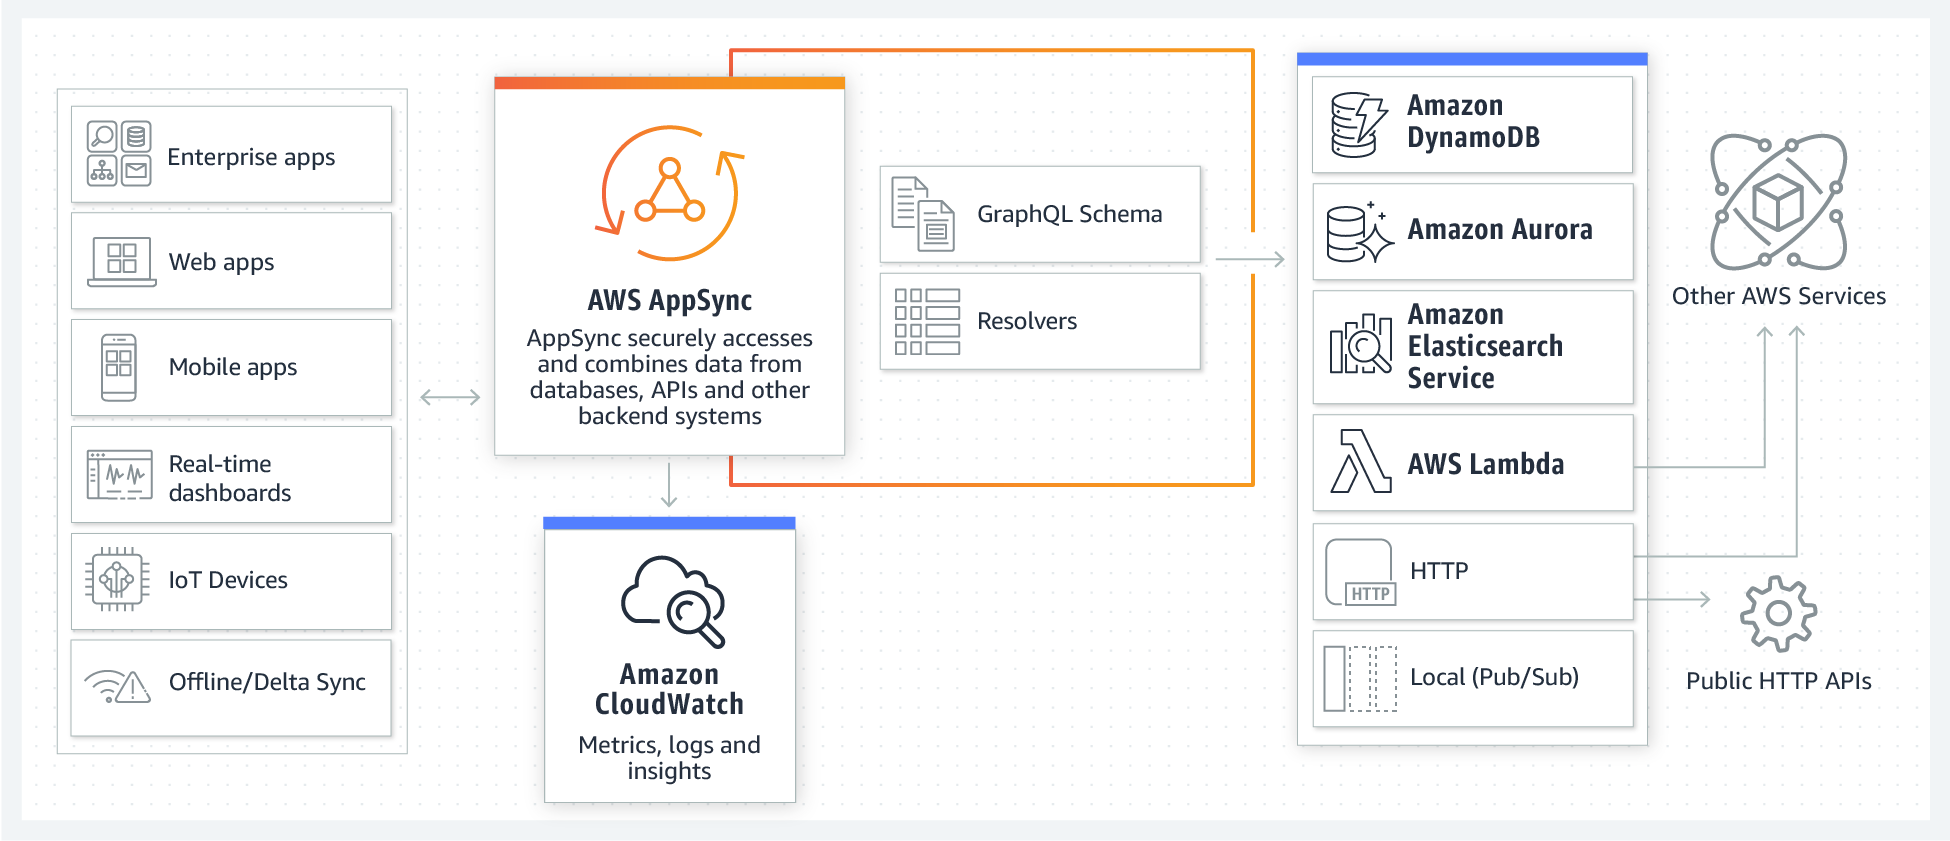
\includegraphics[width=1.0\textwidth]{40-AWS/Appsync.png}
    \caption{Funktionsweise von AppSync. Links befinden sich alle Geräte und Möglichkeiten, um mit AppSync kommunizieren zu können. Die Rechte Seite illustriert alle Dienste und Protokolle mit denen AppSync kommunizieren kann. AppSync dient als zentrale Verbindung zwischen beiden Seiten. \cite{AppSync}}
    \label{fig:meine-grafik}
\end{figure}
\clearpage
\label{GraphQLResolver}
AppSync besteht aus den Hauptkomponenten GraphQL Schema und Resolver.
Damit GraphQL weiß welche Operationen es bei Anfragen durchführen soll, werden Resolver benötigt.
Resolver sind Funktionen, welche bestimmen wie jedes einzelne Feld im Schema weiterverarbeitet wird.
Es ist nicht möglich Resolver direkt im Schema anzugeben, sie müssen außerhalb erstellt werden.
Im Resolver kann angegeben werden, dass eine Funktion, etwa AWS Lambda, aufgerufen werden soll.
Ein DynamoDB-Resolver ist in der Lage alle benötigten DynamoDB-Tabellen inklusive benötigter Berechtigungen aufzusetzen.
Es ist nur notwendig im Schema die Objekttypen festzulegen.
Daraufhin verknüpft der Resolver die Datenbank mit der API und erstellt alle möglichen Queries und Mutationen automatisch.
Infolgedessen ist es mit AppSync nicht notwendig Query-Typen oder Mutations-Typen zu erstellen.
Darüber hinaus ist es möglich auch eigene Resolver zu erstellen, falls dies benötigt wird.

Zusätzlich kann AppSync eine Autorisierung mit dem Dienst AWS Cognito (siehe \textit{\ref{Cognito} \nameref{Cognito}}) ermöglichen.
Die Autorisierung von Clients ist mit API Keys\footnote{Der API Key ist ein Authentifizierungsschlüssel und wird bei jeder Anfrage übertragen. AWS empfiehlt ihn bei AppSync nur für Entwicklungsumgebungen,
da er leicht kompromittierbar ist und keine Aufteilung von Berechtigungen ermöglicht.}, AWS IAM Credentials \footnote{
    AWS IAM steht für Identity Access Management und beschreibt Amazons Dienst zur Identität- und Benutzerverwaltung. Der Dienst erlaubt es Nutzer anzulegen und
    ihnen Berechtigungen zu zuzuweisen.},
    OIDC Tokens \footnote{OIDC steht für OpenID Connect und basiert auf dem OAuth 2.0 Protokoll zur Authentifizierung.
    OAuth 2.0 erlaubt es den Clients die Identität des nutzers zu überprüfen.
    OpenID ermöglicht es mittels eines Tokens sich bei weiteren Diensten Diensten anzumelden die ebenfalls OpenID unterstützen (OpenID Provider).
    Bekanntes Beispiel ist die Option \glqq Mit Google anmelden\grqq{} oder auch \glqq Mit Apple anmelden\grqq.
    Die Tokens zur Authentifizierung (JWT Tokens) der Identität werden verschlüsselt im JSON Format versendet und ermöglichen einen standardisierten Weg zum Anmelden.

          } oder einem AWS
Cognito User Pool (siehe \textit{\ref{Cognito} \nameref{Cognito}}) möglich. \cite{AppSyncAuth}

Sämtliche Protokolldaten sowie Metriken können in dem Dienst AWS CloudWatch Logs\footnote{ Amazon CloudWatch Logs ist ein Überwachungs- und Management-Service, in dem Logs von sämtlichen AWS-Diensten gespeichert und ausgewertet werden können. } gespeichert und ausgewertet werden.

Auch Echtzeitanwendungen können mit AppSync und GraphQL Subscriptions realisiert werden.
Zusätzlich bietet Amazon ein serverseitiges Caching von Daten an, um direkten Zugriff zu reduzieren und die Geschwindigkeit zu erhöhen.
Für das Caching wird der AWS Dienst ElastiCache verwendet, der auf den Speicher Redis\footnote{Redis steht für Remote Dictionary Server und ist ein schneller Datenspeicher der als Cache geeignet ist. Alle Daten liegen bei Redis im Arbeitsspeicher und ermöglichen einen schnellen Zugriff.} basiert.
Um Caching nutzen zu können, ist es notwendig einen Instanztypen mit bestimmter Kapazität auszuwählen.
Ähnlich wie bei der Preisgestaltung von AWS API Gateway, muss der Cache zeitbasiert bezahlt werden.
Der kleinste auswählbare Instanztyp \verb+cache.small+ mit einer vCPU und 1,55 GB Arbeitsspeicher kostet zum Beispiel 0,044 USD pro Stunde.
Eine Millionen API-Aufrufe kosten 4,00 USD, eine Vergünstigung bei mehr Abrufen gibt es im Vergleich zu API Gateway nicht.
\cite{AppSync} \cite{AppSyncPreise}


\clearpage
\subsubsection{Entscheidung}
Für das, in dieser Arbeit gewünschte Projekt, wäre eine Implementierung sowohl mit einer REST API als auch mit GraphQL möglich.
Beide Dienste für die API sind zudem direkt in Amplify (siehe \textit{\ref{Amplify} \nameref{Amplify}}) integriert und benötigen keine separate Konfiguration.

Mit AWS APIGateway müsste man mehrere unterschiedliche Endpunkte konfigurieren und im Frontend einbauen.
Im ersten Schritt würde eine \verb+GET+ Abfrage auf allen Accounts inklusive aller zusätzlichen Daten ausreichen.
Die benötigte Datenbank und alle damit verbundenen Autorisierungen müssten manuell eingerichtet werden.

GraphQL bietet sich an, wenn man mehrere Microservices nutzt und alle in einem Schema konsolidieren möchte.
Umso größer und komplexer die Anwendung wird, desto mehr spielt GraphQL seine Vorteile aus.
Trotz des Wachstums der Daten bleiben die benötigten Konfigurationsänderungen im Vergleich zu REST geringer und übersichtlicher.

Der Umfang der Webanwendung und der benötigten Daten steigt mit zunehmenden Anforderungen.
Je nachdem welcher Endanwender auf die Anwendung zugreift, könnte er einen unterschiedlichen Detailgrad der Daten benötigen.
Für einen groben Überblick reichen etwa die Gesamtkosten aller Cloud Provider.
Will man jedoch die einzelnen Kosten analysieren und ggfs. optimieren sind mehr Daten notwendig.
Da bisher nur bekannt ist welche Daten benötigt werden, jedoch nicht in welchem Detailgrad, ist eine Umsetzung mit GraphQL, also AWS Appsync von Vorteil.
Auf Wunsch kann die Query jederzeit flexibel angepasst werden.

Außerdem wird einem der Aufwand zur Erstellung der Datenbank und des benötigten Resolvers übernommen, sofern DynamoDB genutzt wird.
Das Erstellen aller Queries, Mutationen und Subscriptions übernimmt einem der Dienst ebenfalls, was einen schnellen Einstieg zur Folge hat.
Sobald ein Schema mit Datenstrukturen definiert wurde generiert AppSync automatisch alle möglichen Operationen.
Diese Operationen können dann im Anschluss direkt im Frontend verwendet werden.

Aufgrund der überzeugenderen Integration und höheren Flexibilität wird die Anwendung mit AWS AppSync realisiert, da viele Einstiegshürden von AWS übernommen werden.
Es ist davon auszugehen, dass es keine gravierenden Unterschiede bei den Kosten geben wird.
Zum einen sind die Kosten in einem ähnlichem Verhältnis, zum anderen werden nicht übermäßig viele Anfragen erwartet.





\subsection{Datenbanksystem}
Es gibt zwei unterschiedliche Technologien für die Nutzung von Datenbanken, relationale und nicht-relationale Datenbanken.
Sie variieren in vielen Aspekten und haben abweichende Anwendungsfälle.
Amazon bietet für beide Technologien eigene Dienste an, die im Folgenden genauer betrachtet und verglichen werden.


\subsubsection{Relationale Datenbanken: AWS RDS}

Relationale Datenbanken speichern Daten in Tabellenform ab, wobei einzelne Tabellen in Relation zueinander stehen.
Aus Benutzersicht besteht die Datenbank nur aus Tabellen, die physische Struktur bleibt ihm verborgen.
Zur Vermeidung von unzulässigen Einträgen benötigt eine Tabelle einen Primärschlüssel, der ein eindeutiges Zeilenmerkmal ist.
Um Beziehungen zu anderen Tabellen zu erzeugen, wird ein Fremdschlüssel benötigt, der eine Referenz auf den Primärschlüssel der anderen Tabelle darstellt.
Damit Redundanzen innerhalb einer Datenbank vermieden werden, kann die Datenbank gemäß den Normalisierungsregeln bearbeitet werden.
So wird gewährleistet, dass Daten nicht mehrfach existieren und bei Veränderung dieser Daten keine Anomalien\footnote{Unter Anomalien versteht man ein Fehlverhalten innerhalb von relationalen Datenbanken. Tabellen
mit Spalten gleicher Bedeutung haben einen unterschiedlichen Inhalt. Eine Normalisierung verhindert Anomalien. } auftreten.
Die Datenstrukturen sind voneinander abhängig. Eine Auswertung oder Veränderung der Daten ist in der Regel mit der Datenbanksprache SQL möglich. \cite{Datenbankvergleich}

Der zugehörige Dienst von Amazon heißt RDS (Relational Database Service) und unterstützt sechs Datenbank-Engines. Dazu gehören
PostgreSQL, MySQL, MariaDB, Oracle Database, Microsoft SQL-Server und Amazons eigener Dienst Aurora.
RDS bietet mehrere unterschiedliche Instanztypen an.
Je höher die geforderte Kapazität, desto höher auch der Preis.
Der Instanztyp lässt sich jederzeit anpassen.
Während des Erstellens müssen Zugangsdaten für den Zugriff angegeben werden.
Man erhält keinen direkten Zugang auf die zugrundeliegende Hardware, sondern einen User für den jeweils ausgewählten SQL Service.
Im Falle von MySQL würde nach Erstellen der Instanz ein Endpunkt zur Verfügung stehen, auf den eine Anmeldung per
\begin{lstlisting}[basicstyle=\ttfamily\small, breaklines=true , frame = single, backgroundcolor=\color{flashwhite} ]
  mysql -h <Endpunkt> -u <User> -p <Passwort>
    \end{lstlisting} Befehl möglich ist. SSH-Zugang oder Ähnliches ist bei RDS nicht vorgesehen.
    Das angegebene Beispiel ist typisch für einen Plattform as a Service Dienst.

Eine Hochverfügbarkeit ist möglich, indem man die Option Multi-Availability Zone auswählt und so eine Standby-Instanz in einer anderen Availability Zone bereitsteht.
Hierdurch steigt jedoch auch der Preis. Software-Patches können von dem Dienst automatisch eingespielt werden.
Abweichend als bei DynamoDB gibt es keine direkte Integration von RDS Datenbanken mit Serverless Anwendungen bei AWS.
AWS stellt keine direkte Verknüpfung zwischen GraphQL API und RDS zur Verfügung. Eine Implementierung mittels REST bzw. API Gateway würde eine zusätzliche Lambda-Funktion voraussetzen, welche
die Abfrage gegen eine nicht öffentliche RDS Datenbank ausführt. Wäre die Datenbank im Internet erreichbar müsste das Frontend Credentials besitzen um auf die Datenbank zugreifen zu können.
RDS eignet sich vor allem bei klassischen SQL-basierten Datenbanksystemen. Gibt es Einschränkungen eine bestimmte Datenbank-Engine zu nutzen, bietet sich der Dienst ebenfalls an.
Der Dienstleister Airbnb nutzt RDS zum Beispiel für automatisierte Replikationen und Leistungstests.
Die günstigste RDS Instanz \glqq db.t3.micro\grqq{} mit 1 Kern, 1 GB Arbeitsspeicher und der Open Source Engine MariaDB kostet in Frankfurt mit einer ausgewählten Hochverfügbarkeit 0,04 USD pro Stunde. \cite{RDS}


\subsubsection{Nicht-relationale Datenbanken: AWS DynamoDB}
\label{DynamoDB}

AWS DynamoDB ist ein serverloser Dienst zur Erstellung und Verwaltung nicht-relationaler Datenbanken.
Bei dieser Art von NoSQL(not only SQL)-Datenbanken werden Daten als Key/Value Paare aufgebaut. Daneben gibt es noch weitere Modelle, etwa Graphdatenbanken oder dokumentenorientierte
Datenbanken.

Bei den Key-Value-Datenbanken können neue Paare hinzugefügt werden ohne die gesamte Struktur abändern zu müssen.
Es können verschiedene Daten ohne Konvertierung gemeinsam gespeichert werden.
Die Keys müssen eindeutig sein und sind mit den Primärschlüssel der relationalen Datenbank vergleichbar.
Um eine Skalierung und Hochverfügbarkeit zu ermöglichen, werden die Daten auf alle vorhandenen Systeme kopiert und verteilt. Daher ist es auch problemlos möglich weitere
Server zu verwenden, um eine größere Menge an Daten zu verarbeiten. Dies wird als horizontales Skalieren bezeichnet.
Relationale Datenbanken bieten meist nur eine vertikale Skalierung an, d.h. um die Performance zu erhöhen, muss in der Regel ein leistungsstärkerer Server genutzt werden.
Zur Erhöhung des Lesedurchsatzes besteht jedoch die Option, ein oder mehrere, Read-Replica zu nutzen, die einen parallelen Lesezugriff ermöglichen.

NoSQL Datenbanken unterstützen in der Regel keine ACID-Eigenschaften\footnote{ACID steht für Atomicity, Consistency, Isolation, Durability und bedeutet im Kern, dass
alle Transaktionen konsistent sind.} sondern nutzen das BASE-Modell\footnote{Base steht für Basically Available, Soft State, Eventually Consistent und
stellt die Verfügbarkeit von Daten an eine höhere Stelle als die Konsistenz.}.
Da bei SQL-basierten Datenbanken lesende Abfragen so lange warten bis schreibende Vorgänge beendet sind, bleibt die Konsistenz der Daten erhalten.
NoSQL Datenbanken könnten im Zweifel unterschiedliche Daten zurückgeben, falls noch nicht alles ausgetauscht wurde. \cite{Datenbankvergleich}

Anders als AWS RDS gibt es bei DynamoDB gar keine Möglichkeiten mehr sich bei der Datenbank-Engine anzumelden. Der Dienst wird als Serverless angeboten.
Es müssen keine Kapazitäten im Voraus berechnet werden, da der Dienst automatisch skaliert.
Anwender haben die Option direkt Tabellen anzulegen.
Zudem entfällt es auch sich um Software-Patches oder der Sicherstellung der Hochverfügbarkeit zu kümmern, da Tabellen immer global bereitgestellt werden.
Im Gegensatz zu den meisten NoSQL Datenbanken unterstützt DynamoDB ACID-Transaktionen. Amazon bietet dafür eine eigene API an, die in der Applikation zusätzlich
implementiert werden muss. Insgesamt ist es sehr schnell möglich eine Tabelle mit dem Dienst bereitzustellen. Zudem existiert so gut wie kein Wartungsaufwand,
da Amazon die Verantwortung für die wichtigsten Aspekte übernimmt.\cite{DynamoDB}

Das Preiskonzept für DynamoDB ist sehr granular aufgebaut und bietet zwei unterschiedliche Kapazitätsmodi an. Der Modus \glqq Bereitgestellt\grqq{} bietet sich an,
wenn es bereits möglich ist Anforderungen an die Kapazität zu bestimmen und der Datenverkehr berechenbar ist. Der Preis wird pro Stunde und benötigte Kapazität errechnet.
Auf der anderen Seite ist der Kapazitätsmodus \glqq On-demand\grqq{} für unbekannte Workloads optimiert und skaliert automatisch mit den Anforderungen.
Hier wird der Preis nicht pro Zeiteinheit berechnet, sondern auf Basis der benötigten Schreib- und Leseanforderungen. Je nachdem welchen genauen API-Aufruf man tätigt
kann dieser eine halbe Einheit oder zwei Einheiten erfordern. Zur Option stehen \glqq Strongly Consistent Reads\grqq{} und \glqq Eventually Consistent Reads\grqq { \footnote{ Bei einem Strongly Consistent Aufruf
gibt DynamoDB den aktuellsten Datensatz zurück. Bei Eventually Consistent besteht die Möglichkeit, dass der Wert nicht der aktuellste ist.
Nachteil von Strongly Consistent ist die höhere Latenz und ein höherer Verbrauch der Leseanforderungseinheiten. } DynamoDB nutzt standardmäßig
\glqq Eventually Consistent Reads\grqq , wobei ein Aufruf bis zu 8 KB eine Einheit erfordert.
Eine Million dieser Schreibanforderungen kosten in Frankfurt 1,525 USD und eine Million Leseanforderungen 0,305 USD.
Zudem entstehen Kosten für den Datenspeicher, die Sicherung, Datenübertragung und ein paar weitere speziellere Funktionen.
Beim Datenspeicher sind die ersten 25 GB pro Monat kostenlos und kosten danach pro GB-Monat 0,306 USD. \cite{DynamoDBPreise}
\clearpage
\subsubsection{Entscheidung}
Eine NoSQL-Datenbank, und damit AWS DynamoDB, sind für diese Projektumsetzung besser geeignet.
Zum einen ist der von Amazon zur Verfügung gestellte Dienst besser mit den restlichen Komponenten integriert, zum anderen ist der NoSQL Ansatz
auch durch die höhere Flexibilität passender.
Eine RDS Datenbank müsste separat vom restlichen Workflow aufgesetzt und konfiguriert werden. Egal ob GraphQL API oder REST API, eine Umsetzung mit RDS wäre deutlich
aufwendiger als mit DynamoDB.
Bei der Kombination GraphQL und RDS müsste das GraphQL Schema samt aller Queries und Mutationen manuell erstellt werden, da kein automatisierter
Dienst dafür existiert. Auf der anderen Seite müsste für das API Gateway zusätzlich einen Weg zur Kommunikation mit der RDS Datenbank bereitgestellt werden.
Die Möglichkeit die RDS Datenbank im Internet erreichbar zu machen ist auf Grund des erhöhten Sicherheitsrisikos keine Option.

Der DynamoDB Dienst ist im Vergleich dazu erheblich einfacher aufzusetzen.
Der Workflow der Anwendung benötigt keine ACID-Garantien oder komplexe Abfragen. Beziehungen sind ebenfalls nicht vorhanden, da es sich um Daten unterschiedlicher
Cloud Provider handelt die keinen direkt Bezug zueinander haben.
Mit RDS ist eine Auswahl eines Instanztypes notwendig und es würden ebenfalls pauschale Kosten für die Server anfallen.
Da bereits die Entscheidung für AWS AppSync bei der API fiel, ist es zudem eine erhebliche Erleichterung eine DynamoDB Tabelle mit der API zu verknüpfen.
Eine Umsetzung mit DynamoDB ermöglicht es den Konfigurationsaufwand und die Kosten minimal zu halten.


\subsection{Authentifizierung}
\label{Authentifizierung}
Da die Anwendung bei AWS gehostet wird, wird sie auch über das Internet erreichbar sein.
Um den Zugriff nur für ausgewählte Mitarbeiter der Mediengruppe RTL einschränken zu können ist eine Authentifizierung essentiell.
Ohne Registrierung und Anmeldung darf es nicht möglich sein Daten einzusehen.
Im besten Fall ist es sogar möglich die Authentifizierung mit bereits vorhandenen Firmenidentitäten zu verknüpfen, sodass keine eigenen
Benutzer registriert werden müssen.

Alle Mitarbeiter der Mediengruppe RTL werden in einer eigenen Active Directory Domäne auf On Premises Servern verwaltet.
Dieses Verzeichnis wird mit dem Cloud-Dienst Azure Active Directory synchronisiert.
Dadurch können sich Mitarbeiter von jedem Ort aus authentifizieren und von Single Sign-On (SSO) profitieren.
Mit Single Sign-On benötigt man nur eine einmalige Authentifizierung, um auf sämtliche unterstütze Dienste mit derselben Identität zugreifen zu können.
Der Anwender muss sich nicht mehr überall einzeln anmelden.
Innerhalb des SSO-Systems wird die Identität zusammengeführt und übernimmt die Aufgabe die Identität des Anwenders zu bestätigen.
Größter Vorteil ist eine konsolidierte Möglichkeit zur Anmeldung. Zudem muss der Anwender, falls er das Unternehmen verlässt, nur noch an einer Stelle entfernt werden und der Zugang zu allen Diensten wird automatisch entzogen.
Zusätzlich wird unter bestimmten Bedingungen eine MFA-Verifizierung \footnote{MFA steht für Multi-Factor Authentication und steigert die Sicherheit für Nutzer indem neben dem Passwort
ein weiterer Faktor zum Anmelden benötigt wird. Häufig wird als Zweitfaktor eine SMS mit einem Code oder
ein Einmalkennwort welches mittels TOTP(Time-based One-time Password) Verfahren generiert wird. } erfordert.

Um den Registrierungs- und Anmeldeprozess so einfach wie möglich zu gestalten, bietet AWS den Dienst Cognito an.

\subsubsection{AWS Cognito}
\label{Cognito}
Amazon Cognito ist ein voll integrierter Dienst zur Benutzerverwaltung und Autorisierung.
Cognito übernimmt dabei die Registrierung und Verwaltung neuer Benutzer sowie die Steuerung von Zugriffen.
Mithilfe des AWS Amplify-Frameworks kann die Benutzeroberfläche zum Registrieren bzw. An- und Abmelden leicht in die eigene Anwendung implementiert werden.
Das Framework stellt SDKs für alle gängigen mobilen Plattformen sowie JavaScript inklusive JavaScript-Frameworks wie React, Angular und Vue bereit.
Ein Vergleich der Javascript-Frameworks befindet sich im Abschnitt \textit{\ref{FrontendFramework} \nameref{FrontendFramework}}.
Es soll möglich sein, mit wenig Code die eigene Anwendung mit Cognito zu verknüpfen, und bei Bedarf die Oberfläche anzupassen.
Der Dienst ist vollständig Serverless aufgebaut und bietet die Option \glqq Hunderte von Millionen Benutzern\grqq{} zu verwalten,
\glqq ohne dass Server-Infrastruktur aufgestellt werden muss.\grqq \cite{CognitoUebersicht} \cite{Cognito2}

Cognito besteht aus den Komponenten Benutzerpools und Identitäten-Pools.
Ein Benutzerpool ist ein Verzeichnis durch den Benutzer angelegt und verwaltet werden können.
Hier können Attribute konfiguriert werden, z.B. mit welcher Information sich Benutzer anmelden können.
Zur Option stehen ein Username, die E-Mail Adresse oder eine Telefonnummer.
Außerdem ist es möglich weitere Attribute zu setzen, wie etwa das Geschlecht, der Wohnort, das Geburtsdatum.
Eine Verifizierung mit einem zweiten Faktor ist ebenfalls im Dienst implementiert.
Über den Benutzerpool können ebenfalls App-Clients erstellt werden.
Ein App-Client wird genutzt um nicht authentifizierte Operationen durchführen zu können.
Dazu gehört das Registrieren, Anmelden und die Passwortwiederherstellung.
Es ist möglich mehrere App-Clients zu nutzen, beispielsweise jeweils einen für einen Android, iOS und Webclient.

Der Identitäten-Pool erlaubt es Nutzern Zugriff auf andere Dienste zu erteilen. Es werden eindeutige Identitäten erstellt und diese mit anderen Diensten verbunden.
Dabei unterstützt Cognito soziale Identitätsanbieter wie Google, Facebook oder Apple, aber auch Unternehmens-Identitätsanbieter wie Microsoft Active Directory.
Hierfür werden gängige Standards zur Verwaltung von Identitäten wie OpenID, OAuth 2.0 und SAML 2.0\footnote{SAML steht für Security Assertion Markup Language und ist ein XML-Framework zur  Authentifizierung und Autorisierung.
Anders als bei OpenID Connect, benötigt SAML eine konfigurierte Vertrauensbeziehung. Häufig kommt SAML bei Single Sign-On Verfahren zum Einsatz. } genutzt. \cite{Cognito1}

Ähnlich zu den meisten anderen Serverless Diensten von AWS, fallen auch bei Cognito keine pauschalen Kosten an.
Nur die tatsächliche Nutzung wird in Rechnung gestellt.
Amazon gewährt für die ersten 50.000 monatlich aktiven Benutzer ein kostenloses Kontingent.
Dieses gilt jedoch nur für Benutzer die direkt über den Cognito User Pool oder soziale Identitätsanbieter registriert sind.
Bei Anmeldungen mit einem Unternehmens-Identitätsanbieter liegt das kostenlose Kontingent bei 50 Nutzern.
Darüber hinaus kostet jeder weitere Nutzer 0.0055 USD pro Monat.
Ab einer Anzahl von 100.000 wird der Preis niedriger gestaffelt.
Außerdem können Kosten für die SMS-Nachrichten bei der MFA Authentifizierung anfallen.\cite{CognitoPreise}


\subsubsection{Alternative und Entscheidung}
\label{CognitoEntscheidung}
Da Amazon Cognito alle gängigen Standards zur Authentifizierung unterstützt, wird auch kein alternativer Dienst angeboten.
Alle Möglichkeiten werden bedient und mithilfe des Amplify-Frameworks ist eine Implementierung ebenfalls leicht realisierbar.
Theoretisch ist es nicht einmal notwendig eine eigene Oberfläche zur Anmeldung zu schreiben.

Die einzige alternative Möglichkeit besteht darin, die gesamte Authentifizierung selbstständig zu schreiben.
JavaScript-Frameworks wie React oder Vue können den Prozess etwas erleichtern, nichtsdestotrotz ist der Aufwand deutlich höher als die Verwendung von Cognito.
Der Vorteil einer eigenen Implementierung ist eine höhere Flexibilität und ein größerer Lernprozess, da sich mit allen einzelnen Schritten intensiver befasst werden muss.
Wird gewünscht zusätzlich MFA oder eine sichere Passwortwiederherstellung einzubauen, muss noch mehr Zeit einkalkuliert werden.

Angesichts der enormen Einfachheit und ausreichenden Flexibilität ist die Verwendung von Cognito die sinnvollere Wahl.
Auf Wunsch kann Cognito mit einer Vielzahl von Anbietern und Diensten verknüpft werden, sowie direkt in Amplify integriert werden.
Das Amplify-Framework bietet für die gängigen JavaScript-Frameworks vorgefertigte Module an, um noch weniger Konfigurationsaufwand betreiben zu müssen.
Dank Cognito dürfte die Implementierung einer Authentifizierung in einer Serverless Anwendung keinen allzu großen Aufwand mehr benötigen.


\subsection{Backend Logik}
Um überhaupt Daten erhalten zu können, ist ein Backend-Prozess zum Verarbeiten von Anforderungen erforderlich.
Für die gewünschte Implementierung ist es notwendig eine Liste aller AWS Accounts abzufragen und anschließend diese Daten in die DynamoDB Tabelle abzuspeichern.
Falls notwendig soll auch die Datenstruktur angepasst werden.
Dieser Prozess muss regelmäßig ausgeführt werden, da ständig neue AWS Accounts der Organisation hinzugefügt werden.
Bestenfalls wird der Prozess direkt nach der Erstellung eines neuen Accounts initiiert.

Zur Bewältigung dieser Aufgabe sind die meisten AWS Dienste potenziell einsetzbar, jedoch nicht wirklich geeignet.
Eine EC2 Instanz mit Linux Betriebssystem und Programmcode könnte theoretisch die Datenverarbeitung durchführen, es entspricht jedoch nicht der Serverless Architektur und benötigt signifikant mehr Aufwand in der Umsetzung und Wartung.
Auch eine Docker-basierte Lösung benötigt merklich mehr Arbeit, da die Laufzeitumgebung und Datenverarbeitung weiterhin im Verantwortungsbereich des Nutzers liegt.
Außerdem müsste bei beiden zuvor genannten Optionen mindestens ein Server bzw. Container dauerhaft laufen um Anfragen annehmen zu können.
Beide Varianten sind keine valide Option für eine Serverlose Umsetzung.

Möchte man Code mit einem Minimum an Administrationsaufwand in der Cloud ausführen eignet sich der Dienst AWS Lambda, der im folgenden Abschnitt ausführlicher erläutert wird.

\subsubsection{AWS Lambda}
\label{Lambda}
Im November 2014 wurde der Serverlose Datenverarbeitungsservice AWS Lambda veröffentlicht, mit dem Anwender ihren Code jederzeit ausführen können.
Amazon kümmert sich um die \glqq gesamte Administration der Datenverarbeitungsressourcen, einschließlich der Server- und Betriebssystemwartung, Kapazitätsbereitstellung, automatischen Skalierung sowie der Code-Überwachung und -Protokollierung.\grqq{} \cite{LambdaZitat}
\clearpage
Da auch die Laufzeitumgebung von AWS verantwortet wird, ist die Auswahl der Programmiersprachen vorgegeben.
Zur Auswahl stehen NodeJS, Python, Ruby, Java, Go, C\# und Powershell.
Mit etwas mehr Aufwand ist es zudem auch möglich eine Benutzerdefinierte Laufzeit zu implementieren, sodass weitere Sprachen möglich sind.
NodeJS und Python Code können direkt in der Webkonsole geschrieben und getestet werden.
Weiterhin besteht die Möglichkeit den Code mithilfe einer ZIP-Datei oder über die lokale Entwicklungsumgebungen hochzuladen.\cite{LambdaFAQ}

Wie bereits im Abschnitt \textit{\ref{FaaS} \nameref{FaaS}} erwähnt arbeitet Lambda eventbasiert und kann sowohl von anderen AWS-Diensten, als auch durch einen manuellen Aufruf ausgelöst werden.
Zum einem kann Lambda direkt Daten aus Services lesen, welche einen Datenstrom oder eine Warteschlange erzeugen.
So ist es möglich jedes Mal eine Lambda-Funktion auszulösen, sobald eine DynamoDB-Tabelle aktualisiert wird.
Hierbei liest Lambda die Datensätze selbst und benötigt dementsprechend auch Berechtigungen auf die DynamoDB-Tabelle.\cite{LambdaDynamo}
Eine zweite Variante ermöglicht es bestimmten AWS Diensten eine Lambda-Funktion aufzurufen.
Dienste wie Cognito oder API Gateway können bei Ereignissen die Lambda-Funktion auslösen und warten bis sie eine Antwort erhalten.
Hier findet ein synchroner Aufruf statt.
Anders als bei den Diensten Amazon S3 oder Amazon SES\footnote{SES steht für Simple E-Mail Service und ist ein Dienst zum Versenden und Empfangen von Mails.} findet ein asynchroner Aufruf statt, und die Dienste warten nicht auf eine erfolgreiche Antwort.
Sie erfahren nur, dass Lambda das Ereignis in eine Warteschlange übergeben hat.
Falls bei der Übergabe Fehler auftreten, kann die Funktion erneut ausgeführt werden.
Alle Informationen zur Lambda-Funktion, auch potenzielle Fehler im Code, werden automatisch protokolliert und in Amazon CloudWatch Logs gespeichert.
\cite{LambdaDienste}

Sobald eine Lambda-Funktion ausgelöst wird, startet die Codeausführung am sog. Handler.
Der Handler ist eine spezielle Methode innerhalb des Lambda-Codes der Ereignisse verarbeitet.
Je nach Programmiersprache existieren unterschiedliche Voraussetzungen.
In dem Handlers können weitere Funktionen und Methoden aufgerufen werden die zur Bearbeitung notwendig sind.
Wenn der Handler mit der Ausführung des Codes fertig ist, steht er für weitere Events zur Verfügung.
Werden mehrere Events ausgelöst, starten auch gleichzeitig mehrere Kopien der Funktion.
Nach dem Fertigstellen skaliert Lambda automatisch bis keine Ressourcen im Leerlauf übrig bleiben.
Um eine fehlerfreie Ausführung von beliebig vielen Funktionen sicherzustellen, ist die Zustandslosigkeit somit essentiell.
Dies bedingt ebenfalls, dass der Speicherplatz nicht persistent ist und auf 500 MB eingeschränkt ist.\cite[Seite 5f]{AWSWhitepaper}

Während der Erstellung einer Funktion wird zusätzlich eine Lambda-Ausführungsrolle mit Berechtigungen definiert.
Diese Ausführungsrolle gewährt der Funktion Zugriff auf Dienste und Ressourcen die angegeben worden sind.
Die Berechtigungen können dabei jederzeit ergänzt oder entfernt werden.
Dank der Ausführungsrolle ist es möglich die Zugriffskontrolle nach dem Least-Privilege-Prinzip\footnote{Durch das Least-Privilege-Prinzip wird sichergestellt, dass nur die minimal erforderlichen Berechtigungen zugeteilt werden. } zu konzipieren.

Damit ein Fehler im Code eine Lambda-Funktion nicht theoretisch unendlich lang laufen lässt, wird die Funktion nach maximal 15 Minuten terminiert.
Außerdem ist es nicht möglich einer Funktion beliebig viele Ressourcen zuzuteilen.
Amazon erlaubt aktuell maximal 3 GB an Arbeitsspeicher und minimal 128 MB.
Die Größe des Arbeitsspeichers muss selbst ausgewählt werden.
\clearpage
Bezahlt wird bei Lambda die Dauer der Ausführung sowie die Anzahl der Anforderungen.
Die Dauer wird in 100-Millisekunden-Schritten berechnet und der Preis ist je nach Größe des Arbeitsspeichers abhängig.
512 MB Arbeitsspeicher kosten etwa 0,0000008333 USD pro 100ms.
Anforderungen, zu denen jeder Aufruf oder jede Ereignisbenachrichtigung zählen, kosten 0,20 USD pro 1 Mio. Anforderungen.\cite{LambdaPreise}

\subsubsection{Entscheidung}
\label{LambdaEntscheidung}
AWS Lambda eignet sich optimal zur Realisierung der Webanwendung.
Direkt nach Erstellung der Lambda-Funktion und setzen der passenden Berechtigungen, kann am Code geschrieben werden.
Dementsprechend muss keine Zeit für Themen wie Netzwerk, Virtualisierung oder die Laufzeitumgebung vergeudet werden.

Für die Webanwendung wird eine Lambda-Funktion benötigt, die über den Dienst AWS Organizations alle zurzeit verfügbaren Accounts abrufen kann.
AWS Organizations ist ein zentraler Dienst zur Steuerung und Verwaltung von AWS Accounts.
Innerhalb eines Master-Accounts werden neue Accounts nach Bedarf erstellt und konfiguriert.
Nur dieser Master-Account besitzt Informationen über alle verfügbaren Accounts in der Organisation.
Die Lambda-Funktion, welche in einem anderen Account bereitgestellt wird, benötigt Zugriff auf den Master-Account und muss über eine API die Liste der Accounts abrufen können.
Anschließend müssen die gesammelten Daten in die DynamoDB-Tabelle gespeichert werden.
Alle Komponenten dieses Projektes werden in einem separaten Account erzeugt, der durch die Organisation erstellt wurde.

Da das Frontend mit einem JavaScript-Framework erzeugt wird, bietet es sich an für Lambda NodeJS als Programmiersprache zu verwenden.
So wird vermieden zwei unterschiedliche Syntaxstrukturen und Funktionsweisen lernen zu müssen.
AWS bietet für NodeJS eine AWS Organizations API an, um exakt diesen Aufruf tätigen zu können.
Der Abschnitt \textit{\ref{ImpLambda} \nameref{ImpLambda}} beschreibt die exakte Implementierung mit NodeJS und dessen Herausforderungen.

Der Zugriff auf AWS Organizations sowie die Accountstruktur der Mediengruppe RTL werden im Abschnitt \textit{\ref{Accountstruktur} \nameref{Accountstruktur}} genauer erläutert.
\cite{SDKListAccounts}

\subsection{Frontend Framework}
\label{FrontendFramework}
Die bisher ausgewählten Dienste Cognito und AppSync unterstützten die gängigsten JavaScript-Frameworks.
Auch im Zusammenspiel mit Amplify gibt es keine Einschränkungen.
Zur Auswahl für das Web-Frontend wurden React, React Native, Vue und Angular betrachtet.
React Native eignet sich nicht zur Umsetzung, da es hauptsächlich für die native Entwicklung von iOS und Android Apps genutzt wird.
Mit allen drei restlichen Frameworks lässt sich das Frontend mit einem ähnlichen Aufwand aufbauen.
Die Entscheidung erfolgt anhand von Aspekten wie Syntax, Popularität und Performance.
\clearpage
Angular wurde 2010 von Google entwickelt und ist das älteste der drei JavaScript-Frameworks.
Für die Syntax verwendet Angular TypeScript
\footnote{TypeScript ist eine von Microsoft entwickelte Erweiterung oder auch Überkategorie von JavaScript.
Mit TypeScript generierter Code lässt sich in JavaScript kompilieren. Im Gegensatz zu JavaScript muss bei TypeScript jede Variable einen Typ zugewiesen bekommen.
 } in Kombination mit HTML.
 Angular gehört mit React zu den verbreitesten Frameworks und bietet viele themenbezogene Beiträge auf Plattformen wie Stack Overflow\footnote{Stack Overflow ist eine Internetseite auf der Benutzer Fragen und Antworten rund um das Thema Programmierung und Softwarentwicklung stellen können. } und weiteren.
 Aufgrund der ungleichen Syntax zu JavaScript und dem daraus resultierenden mutmaßlich schwereren Einstieg scheint Angular nicht die beste Lösung zu sein.
 Dementsprechend ist die Entscheidung nicht auf Angular gefallen.

Vue ist mit Veröffentlichung im Jahr 2014 das jüngste Framework und wird von keinem großen Unternehmen, sondern durch die Community weiterentwickelt.
In den letzten Jahren ist Vue zunehmend populärer geworden und mittlerweile existieren auch vermehrt Standardbeispiele zum Erstellen von Webanwendung.
Besonders in China ist Vue sehr verbreitet.\cite[Abschnitt: Comparing Adoption \& Popularity]{JavascriptFrameworks}
Code wird mithilfe von JavaScript und HTML geschrieben und dabei strikt voneinander getrennt.
Der HTML Code befindet sich im \verb+<template>+ Bereich und JavaScript Code ist im \verb+<script>+ Bereich erlaubt.
Hinsichtlich der geringeren Verbreitung im englischsprachigen Raum und dem geringeren Reifegrad der AWS-Integration, wird Vue nicht für die Realisierung verwendet.

React wurde 2013 von Facebook veröffentlicht und wird zusammen mit der Community weiterentwickelt.
Anders als bei Vue, findet keine solche Trennung statt.
React arbeitet, wie die meisten JavaScript-Frameworks, komponentenbasiert und versucht die Komponenten modular zu strukturieren.
Zum Rendern von HTML Elementen nutzt React die JavaScript-Erweiterung JSX, welche JavaScript und HTML Syntax kombiniert.
Der JSX Code wird vor dem Start der Anwendung in normalen Javascript-Code übersetzt.
Innerhalb von geschweiften Klammern wird alles als Javascript Code behandelt.
Es ist also auch möglich alle Elemente direkt mit React und Javascript zu erzeugen, jedoch versucht JSX eine komfortablere und leichtere Lösung anzubieten.
Anstatt Methoden wie \verb+React.createElement()+ zu nutzen reicht es aus die HTML Syntax zu kennen.
Mit JSX lässt sich ein \verb+<div>+ Element wie folgt erzeugen:
\begin{lstlisting}[basicstyle=\ttfamily, breaklines=true , frame = single, backgroundcolor=\color{flashwhite} ]
const divelement = <div>Ich bin ein DIV-Element</div>;

ReactDOM.render(divelement, document.getElementById('root'));
\end{lstlisting}

Ohne JSX wäre folgender Code notwendig.\cite{JSX}
\begin{lstlisting}[basicstyle=\ttfamily, breaklines=true , frame = single, backgroundcolor=\color{flashwhite} ]
const divelement = React.createElement('div', {}, 'TEXT');

ReactDOM.render(divelement, document.getElementById('root'));
\end{lstlisting}


Da im Studium bereits Erfahrung mit HTML und JavaScript gemacht wurde, ist der Einstieg in JSX und React der komfortabelste.
Auch existieren am meisten Referenzen zu React im Zusammenspiel mit AWS, sodass im Problemfall eine Lösungssuche am aussichtsreichsten ist.
Aus diesen Gründen wird die Implementierung in React erfolgen.


\subsection{AWS Amplify}
\label{Amplify}

Amplify ist ein zentraler Dienst rund um das Thema Serverless Webanwendungen, die Veröffentlichung war im November 2017.
Amazon bezeichnet Amplify selbst als {}\glqq ein Set aus Tools und Services, das Entwicklern erlaubt, skalierbare vollständige
mobile und Front-End-Anwendungen zu entwickeln, powered by AWS.\grqq{}\cite{AWSAmplify}

Amplify kann als übergeordnete Einheit angesehen werden, welche alle zuvor erläuterten Dienste an einem Ort zusammenfasst und verwaltet.
Dank Amplify soll es nicht mehr notwendig sein, Dienste einzeln zu erstellen und manuell miteinander zu verknüpfen.
Zusätzlich bietet Amplify die Option für ein statisches Web-Hosting an.
Es ist nur notwendig den Code für die Anwendung entweder über die Web-Konsole oder die CLI hochzuladen.
Den gesamten Workflow für die Bereitstellung kann im Anschluss von Amplify übernommen werden.
Dafür wird eine eigene \spverb+amplifyapp.com+-Subdomäne bereitgestellt.
Diese lässt sich auch auf eine Wunsch-Domain anpassen.
Außerdem besteht die Möglichkeit Amplify mit GitHub zu verknüpfen und somit einen automatisierten CI/CD Workflow aufzubauen.
Sobald ein Code in einem bestimmten Repository aktualisiert wurde, kann Amplify die Anwendung automatisch aktualisieren und veröffentlichen.
 \cite{AmplifyHosting}

Amplify lässt sich sowohl über die Amazon Web Console, als auch über eine eigene Amplify CLI konfigurieren.
Alle verfügbaren Dienste sind in der Amplify Bibliothek vereint und können in das Frontend eingebaut werden.
Das Amplify Framework lässt sich in drei Komponenten unterteilen: Bibliotheken, UI-Komponenten und eine CLI Toolchain.
Jede Komponente kann einzeln oder gemeinsam genutzt werden.

Bibliotheken sind Open Source und nutzen bereits vorhandene AWS Dienste, um eine native Webanwendung für die Cloud bereitzustellen.
Hierzu zählen unter anderem Module für zuvor erwähnte Dienste wie Cognito, AppSync, API Gateway, oder S3.
Darüber hinaus existieren auch Module für Chatbots, Push Benachrichtungen, AR/VR, künstliche Intelligenz sowie weitere.

Auch die UI-Komponenten sind Open Source und sollen eine einfache Verzahnung zwischen dem User Interface und den Workflows der Dienste anbieten.
So gibt es zum Beispiel fertige Interface Elemente für das Hochladen von Bildern und Dateien in S3.

Die Amplify CLI Toolchain dient dazu, ein Serverless Backend zu erstellen und zu verwalten.
Dazu gehört die Erstellung aller zuvor genannten Dienste und Funktionen.
Zudem ist es möglich ein statisches Hosting einzurichten.
Dabei werden die benötigten Daten über ein S3 Bucket bereitgestellt.

Amplify erleichtert es einem Projekte als Full Stack Developer\footnote{Als Full Stack Developer wird jemand bezeichnet, der sowohl Client als auch Server
erstellen und betreuen kann. Er ist allein Verantwortlich für das Frontend, Backend und eventuell damit verbundene Datenbanken.} zu realisieren.
Aus demselben Grund ist die Erstellung eines Prototypen ebenfalls schneller realisierbar.
Neben dem statischen Hosting bietet Amplify vor allem den großen Mehrwert alle benötigten Dienste zentral verwalten zu können.
Dies führt zu einer besseren Übersicht und einem einfacheren Einstieg in die Realisierung.
 \cite{AWSAmplifyKomponenten}


 Nachdem nun alle Dienste vorgestellt wurden und das Design entschieden wurde, wird im kommenden Kapitel die Implementierung durchgeführt.
 Auf Basis der bisher gesammelten Erkenntnisse kann ein Architekturbild entwickelt werden, um die Zugehörigkeit aller Komponenten zu verdeutlichen.
 Im Anschluss folgt die Implementierung inklusive Codebeispielen.
